\chapter{2次元共形場理論での分離クエンチ}\label{chap:singlquench}
\textbf{量子クエンチ(quantum quench)}とは、量子系の平衡状態$\rho$を用意して系のハミルトニアンのパラメータを瞬時に変化させることを指す。クエンチによってハミルトニアンが$H\to H'$と変わるため、一般には$\rho$は$H'$の平衡状態ではなくなり、$t\to \infty$で$H'$に対する平衡状態$\rho'$へ熱平衡化していく。このようなクエンチの問題設定は、孤立量子系の熱平衡化を調べる具体例の一つとして理論的に研究されてきた。近年の実験技術の発展により、冷却原子系を用いて孤立量子系を実現することが出来るようになって以降、様々な量子クエンチに対する系のダイナミクスの研究が理論・実験の双方からなされている。

2次元共形場理論の平衡状態を用意してクエンチしたときのエンタングルメントエントロピーの時間発展を調べる研究は、Calabrese,Cardy\cite{Calabrese2006}によって始まった。エンタングルメントエントロピーは部分系のエネルギー期待値と自由エネルギーの差なので、これを調べることでエンタングルメントによって生じた系の熱力学的なダイナミクスを調べることができる。特に、強結合な2次元共形場理論をクエンチしたときのエンタングルメントエントロピーの解析は、カオス性の強い系の平衡化を考える上でも興味深いが、一般には解析が難しい問題である。そこでAdS/CFT対応や笠-高柳公式を通して、AdS時空での測地線のダイナミクスに置き換えると、エンタングルメントエントロピーの時間発展を簡単に計算できるようになる。

この章では我々の研究\cite{Shimaji:2018czt}に基づき、直線上の共形場理論の真空を分離クエンチしたときのエンタングルメントエントロピーの時間発展を調べる。分離クエンチは実験的にも調べられており\cite{gring2012relaxation}、現実の系への応用を考える上でも興味深い。

\ref{sec:SPQsetup}節ではレプリカ法による計算のセットアップを説明し、\ref{sec:SPQdirac}節で零質量自由Dirac場での計算をする。そして\ref{sec:SPQholcft}節で重力双対を持つような2次元共形場理論でのエンタングルメントエントロピーの時間発展を計算し、AdS時空内の測地線を用いてその振る舞いを解釈する。

\section{問題設定}\label{sec:SPQsetup}
2次元共形場理論における分離クエンチとは、空間方向の1点での相互作用を時刻$t=0$で瞬時に``切る''ことを指す。切られた部分を境界として、分離によって因果的に独立な2つの領域$L,R$が生じる(図\ref{fig:sqlorentz})。
\begin{figure}[h]
	\centering
	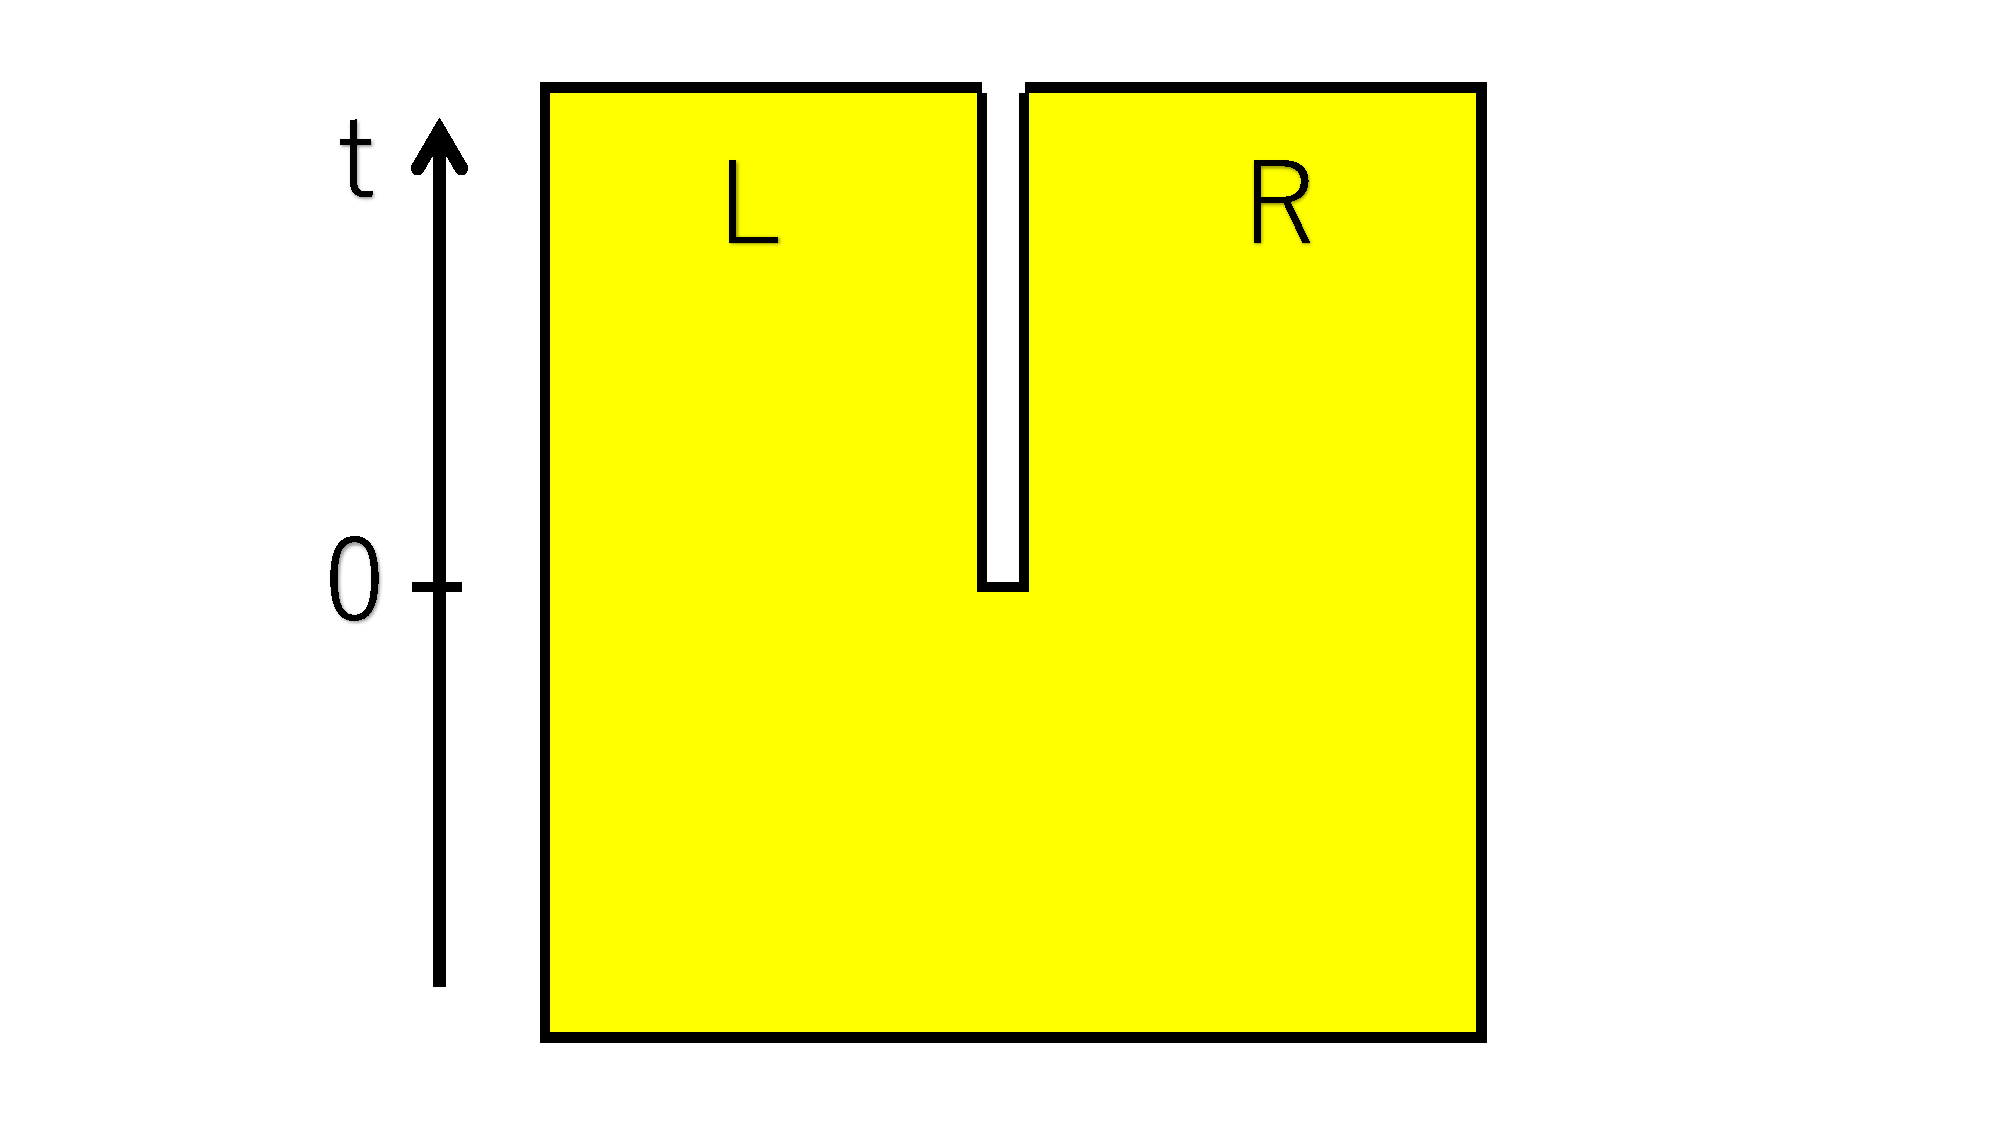
\includegraphics[width=0.7\linewidth]{SQlorentz.pdf}
	\label{fig:sqlorentz}
	\caption{分離クエンチされた系の図。分離によって因果的に独立な2つの領域$L,R$が生じる。}
\end{figure}

真空を分離クエンチした状態に対するエンタングルメントエントロピーをレプリカ法で計算するには、虚時間$\tau=-0,+0$面にクエンチされた状態$|\Psi\ra, \la\Psi|$を経路積分で用意して、注目系以外をトレースアウトしてorbifoldを作る。そして、実時間でのエンタングルメントエントロピーを得るには、レプリカ法で得た虚時間のエンタングルメントエントロピーの結果を$\tau\to 0+it$と解析接続する。

虚時間での経路積分は、区間$[-ia,ia]$に分離が入った平面$w=x+i\tau$座標(図\ref{fig:sqmapping})に対して行う。
\begin{figure}[h]
	\centering
	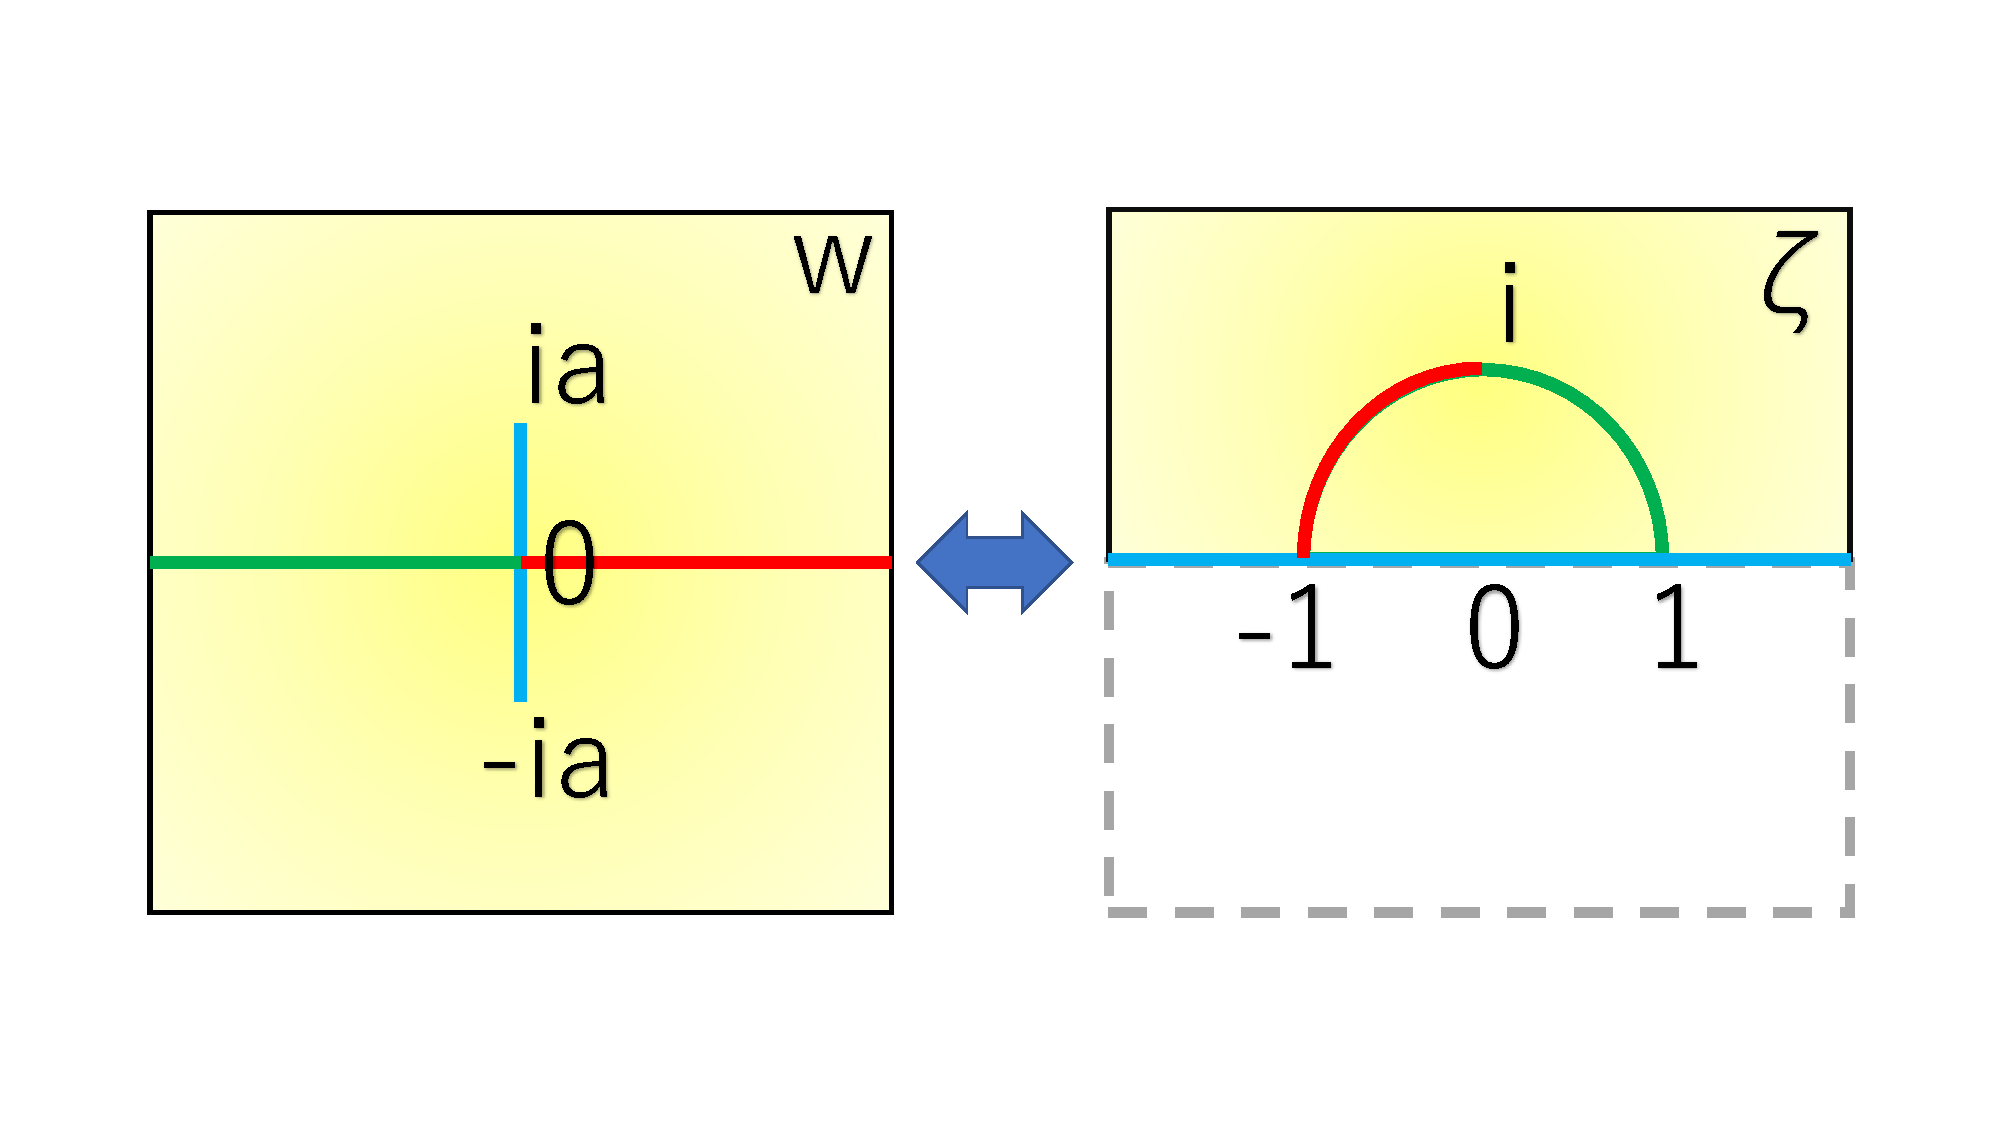
\includegraphics[width=0.7\linewidth]{SQmapping.pdf}
	\label{fig:sqmapping}
	\caption{左は分離クエンチされた真空についてのレプリカ法のセットアップの図。これを共形変換することで右の上半平面に移る。}
\end{figure}

$w$座標は共形変換
\begin{align}
\zeta=i\sqrt{\frac{w+ia}{w-ia}}\equiv f(w)
\end{align}
によって上半平面に移る。したがって虚時間でのエンタングルメントエントロピーの計算は、上半平面$\zeta$上に挿入されたツイスト演算子の相関関数を計算することに帰着される。

ここで、上の共形変換の根号を外すと、
\begin{align}
\zeta(x,\tau)&=\frac{-\ \text{sign}(x)\sqrt{A_{-}(x^2,\tau^2)}+i\sqrt{A_{+}(x^2,\tau^2)}}{\sqrt{2\left(x^2+(\tau-a)^2\right)}}\\
R(x^2,\tau^2)&=\sqrt{(x^2+\tau^2-a^2)^2+4a^2 x^2}\notag\\
&=\sqrt{(x^2+(\tau+a)^2)(x^2+(\tau-a)^2)}\\
A_\pm(x^2,\tau^2) &= R(x^2,\tau^2)\pm(x^2+\tau^2-a^2)
\end{align}
と書けて、さらに微分の絶対値は
\begin{align}
\left| \frac{d\zeta}{dw} \right|=\frac{a}{(R(x^2,\tau^2))^{1/2}\sqrt{x^2+(\tau-a)^2}}
\end{align}
となることに注意しておく。また、$R,A_\pm$は$\tau^2$のみに依存するので、$\tau\to it$の解析接続はそのまま実行できる。このとき、$a \downarrow 0$の極限で
\begin{align}
R(x^2,-t^2)&\sim |x^2-t^2|+\frac{x^2+t^2}{|x^2-t^2|}a^2  \\
A_{\pm}(x^2,-t^2)&\sim \left( |x^2-t^2|\pm (x^2-t^2) \right)+\left( \frac{x^2+t^2}{|x^2-t^2|}\mp 1 \right)a^2
\end{align}
と近似できることに注意しておく。これらの表式は後で使う。

\section{自由ディラック場}\label{sec:SPQdirac}
\subsub{解析計算}
共形境界条件としてNeumann境界条件またはDirichlet境界条件を考える。二重化のトリックを使うと下半平面に鏡像が現れ、Neumann/Dirichlet境界条件に応じてGreen関数は(\ref{scalarGreenUHP}),(\ref{scalarGreenCylinder})となるから、ツイスト演算子は境界条件を反映して
\begin{align}
&&&\text{Neumann}&\sigma_k(\zeta,\overline{\zeta})&=e^{i\frac{k}{n}(X_L(\zeta)-X_R(\overline{\zeta}))}\notag\\
&&&&&=V_{(k/n,-k/n)}(\zeta,\overline{\zeta})&&\left(k=-\frac{n-1}{2},-\frac{n-3}{2},\cdots \frac{n-1}{2}\right)\\
&&&\text{Dirichlet}&\sigma_k(\zeta,\overline{\zeta})&=e^{i\frac{k}{n}(X_L(\zeta)+X_R(\overline{\zeta}))}\notag\\
&&&&&=V_{(k/n,k/n)}(\zeta,\overline{\zeta})&&\left(k=-\frac{n-1}{2},-\frac{n-3}{2},\cdots \frac{n-1}{2}\right)
\end{align}
となる。

区間$[x_1,x_2]$に対するエンタングルメントエントロピーは上のツイスト演算子の2点関数を計算すればよく、NeumannとDirichletで同じ結果が得られる。
\begin{align}
S_A&=-\frac{1}{6}\log (F\epsilon^2)\\
F&=\left|\frac{d\zeta_1}{dw_1}\right|\left|\frac{d\zeta_2}{dw_2}\right|
\frac{(\zeta_1-\overline{\zeta}_2)(\overline{\zeta}_1-\zeta_2)}{|\zeta_1-\overline{\zeta}_1||\zeta_2-\overline{\zeta}_2|(\zeta_1-\zeta_2)(\overline{\zeta}_1-\overline{\zeta}_2)}
\end{align}

いま
\begin{align}
Q(x_1^2,x_2^2,\tau^2)&= \sqrt{(x_1^2+(\tau-a)^2)(x_2^2+(\tau+a)^2)}+(x_1\leftrightarrow x_2)\\
&=\sqrt{2}\sqrt{(x_1^2+\tau^2+a^2)(x_2^2+\tau^2+a^2)-4a^2\tau^2+R(x_1^2,\tau^2)R(x_2^2,\tau^2)}
\end{align}
と書くと、
\begin{align}
|\zeta_1-\zeta_2|^2&=\frac{ Q-\text{sign}(x_1x_2)\sqrt{A_{-1}A_{-2}}-\sqrt{A_{+1}A_{+2}} }{\sqrt{x_1^2+(\tau-a)^2}\sqrt{x_2^2+(\tau-a)^2}}\\
|\zeta_1-\overline{\zeta}_2|^2&=\frac{ Q-\text{sign}(x_1x_2)\sqrt{A_{-1}A_{-2}}+\sqrt{A_{+1}A_{+2}} }{\sqrt{x_1^2+(\tau-a)^2}\sqrt{x_2^2+(\tau-a)^2}}\\
|\zeta_1-\overline{\zeta}_1|&=\frac{\sqrt{2}\sqrt{A_{+1}}}{\sqrt{x_1^2+(\tau-a)^2}}
\end{align}
である。したがって$S_A$は$\tau^2$のみの関数として書けて、
\begin{align}
S_A=\frac{1}{6}\log \left( \frac{2R_1^{1/2}R_2^{1/2}A_{+1}^{1/2}A_{+2}^{1/2}(Q-\text{sign}(x_1x_2)\sqrt{A_{-1}A_{-2}}-\sqrt{A_{+1}A_{+2}})}{a^2\epsilon^2(Q-\text{sign}(x_1x_2)\sqrt{A_{-1}A_{-2}}+\sqrt{A_{+1}A_{+2}})} \right)
\end{align}
となり、解析接続$\tau\to it$はそのまま実行される。いま$|x_1|<|x_2|$として、$a\downarrow 0$の極限をとれば
\begin{align}
Q(x_1^2,x_2^2,-t^2)&\sim \sqrt{2}\sqrt{|(x_1^2-t^2)(x_2^2-t^2)|+(x_1^2-t^2)(x_2^2-t^2)+Q_2 a^2}\\
Q_2&=(x_1^2+t^2)\left(1+\frac{|x_2^2-t^2|}{|x_1^2-t^2|}\right)+(x_1\leftrightarrow x_2)
\end{align}
より、$a\downarrow 0$の極限での$S_A$の近似式は
\begin{align}
S_A(t)\sim \left\{ \begin{array}{ll}
\bigskip\dfrac{1}{3}\log\dfrac{|x_2-x_1|}{\epsilon}  &(0<t<|x_1|)\\
\bigskip\dfrac{1}{6}\log \dfrac{4|x_1|(x_2-x_1)(t-|x_1|)(x_2^2-t^2)}{(x_1+x_2)(t+|x_1|)a\epsilon^2} &(|x_1|<t<|x_2|)\\
\bigskip\dfrac{1}{6}\log \dfrac{4|x_1||x_2|(x_2-x_1)^2}{\epsilon^2(x_1+x_2)^2}  &(|x_2|<t,\ x_1x_2>0 )\\
\dfrac{1}{6}\log\dfrac{4|x_1||x_2|}{\epsilon^2} &(|x_2|<t,\ x_1x_2<0 )
\end{array}\right.
\end{align}
となる。とくに$t\to \infty$では
\begin{align}
S_A(t\to\infty) \sim \left\{ \begin{array}{ll}
\bigskip\dfrac{1}{6}\log \dfrac{4|x_1||x_2|(x_2-x_1)^2}{\epsilon^2(x_1+x_2)^2}  &(x_1x_2>0)\\
\dfrac{1}{6}\log\dfrac{4|x_1||x_2|}{\epsilon^2} &(x_1x_2<0)
\end{array}\right.
\end{align}
となる。

\subsub{数値計算}
上の計算を数値計算したものがグラフ\ref{fig:sd005}である。$a=0.05$で$S_A(t)$と真空のEE $S_\text{vac}=(1/3)\log(L/\epsilon)$の差$S_A(t)-S_\text{vac}$を計算しており、左図は部分系$[50,150]$,右図は$[-20,50]$にとった場合である。
\begin{figure}[h]
	\centering
	\begin{tabular}{c}
		\begin{minipage}{0.50\hsize}
			\centering
			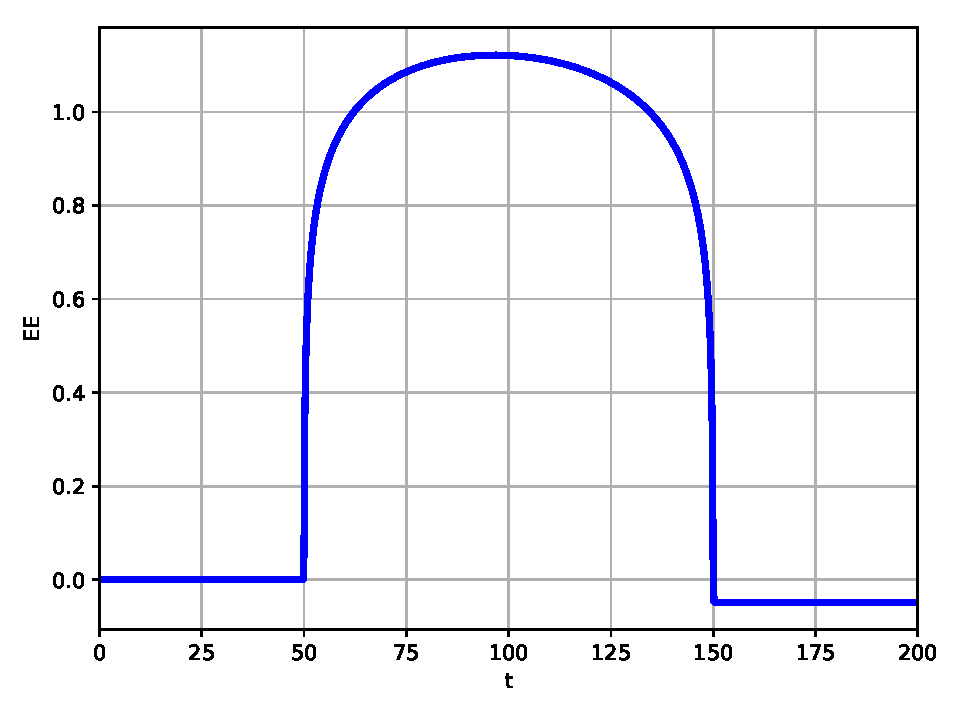
\includegraphics[width=\linewidth]{sd005_50_150.pdf}
		\end{minipage}
		\begin{minipage}{0.50\hsize}
			\centering
			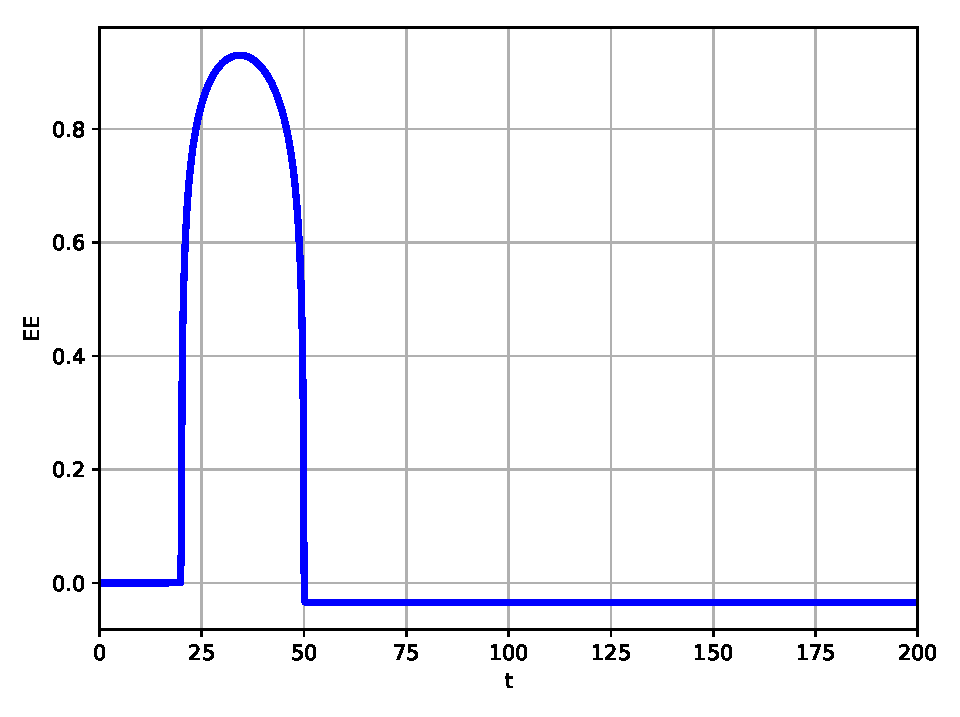
\includegraphics[width=\linewidth]{sd005_20_50.pdf}
		\end{minipage}
	\end{tabular}
	\caption{自由Dirac場の真空を分離クエンチしたときのEEのグラフ。横軸は時間$t$で、縦軸は真空の寄与を引いたEE $S_A(t)-S_\text{vac}$をプロットしている。}
	\label{fig:sd005}
\end{figure}
この結果は\cite{Calabrese:2007rg}で予想されたような、準粒子描像に当てはまっている。

\section{重力双対を持つ共形場理論}\label{sec:SPQholcft}
\subsection{AdS/BCFTの処方を用いたEEの解析}
\subsub{解析計算}
重力双対を持つ共形場理論でのエンタングルメントエントロピーは、笠・高柳公式やHRT公式を用いてAdS空間内の測地線の長さとして計算する。

いま$\zeta$座標は上半平面で定義されている。AdS/BCFTの処方から、$\zeta$座標に対応する境界付きAdS空間としてPoincare座標の上半分を考えることができる。このとき$\IM \zeta=0$面が境界$Q$になる(図\ref{fig:SQadsbcft})。
\begin{figure}[h]
	\centering
	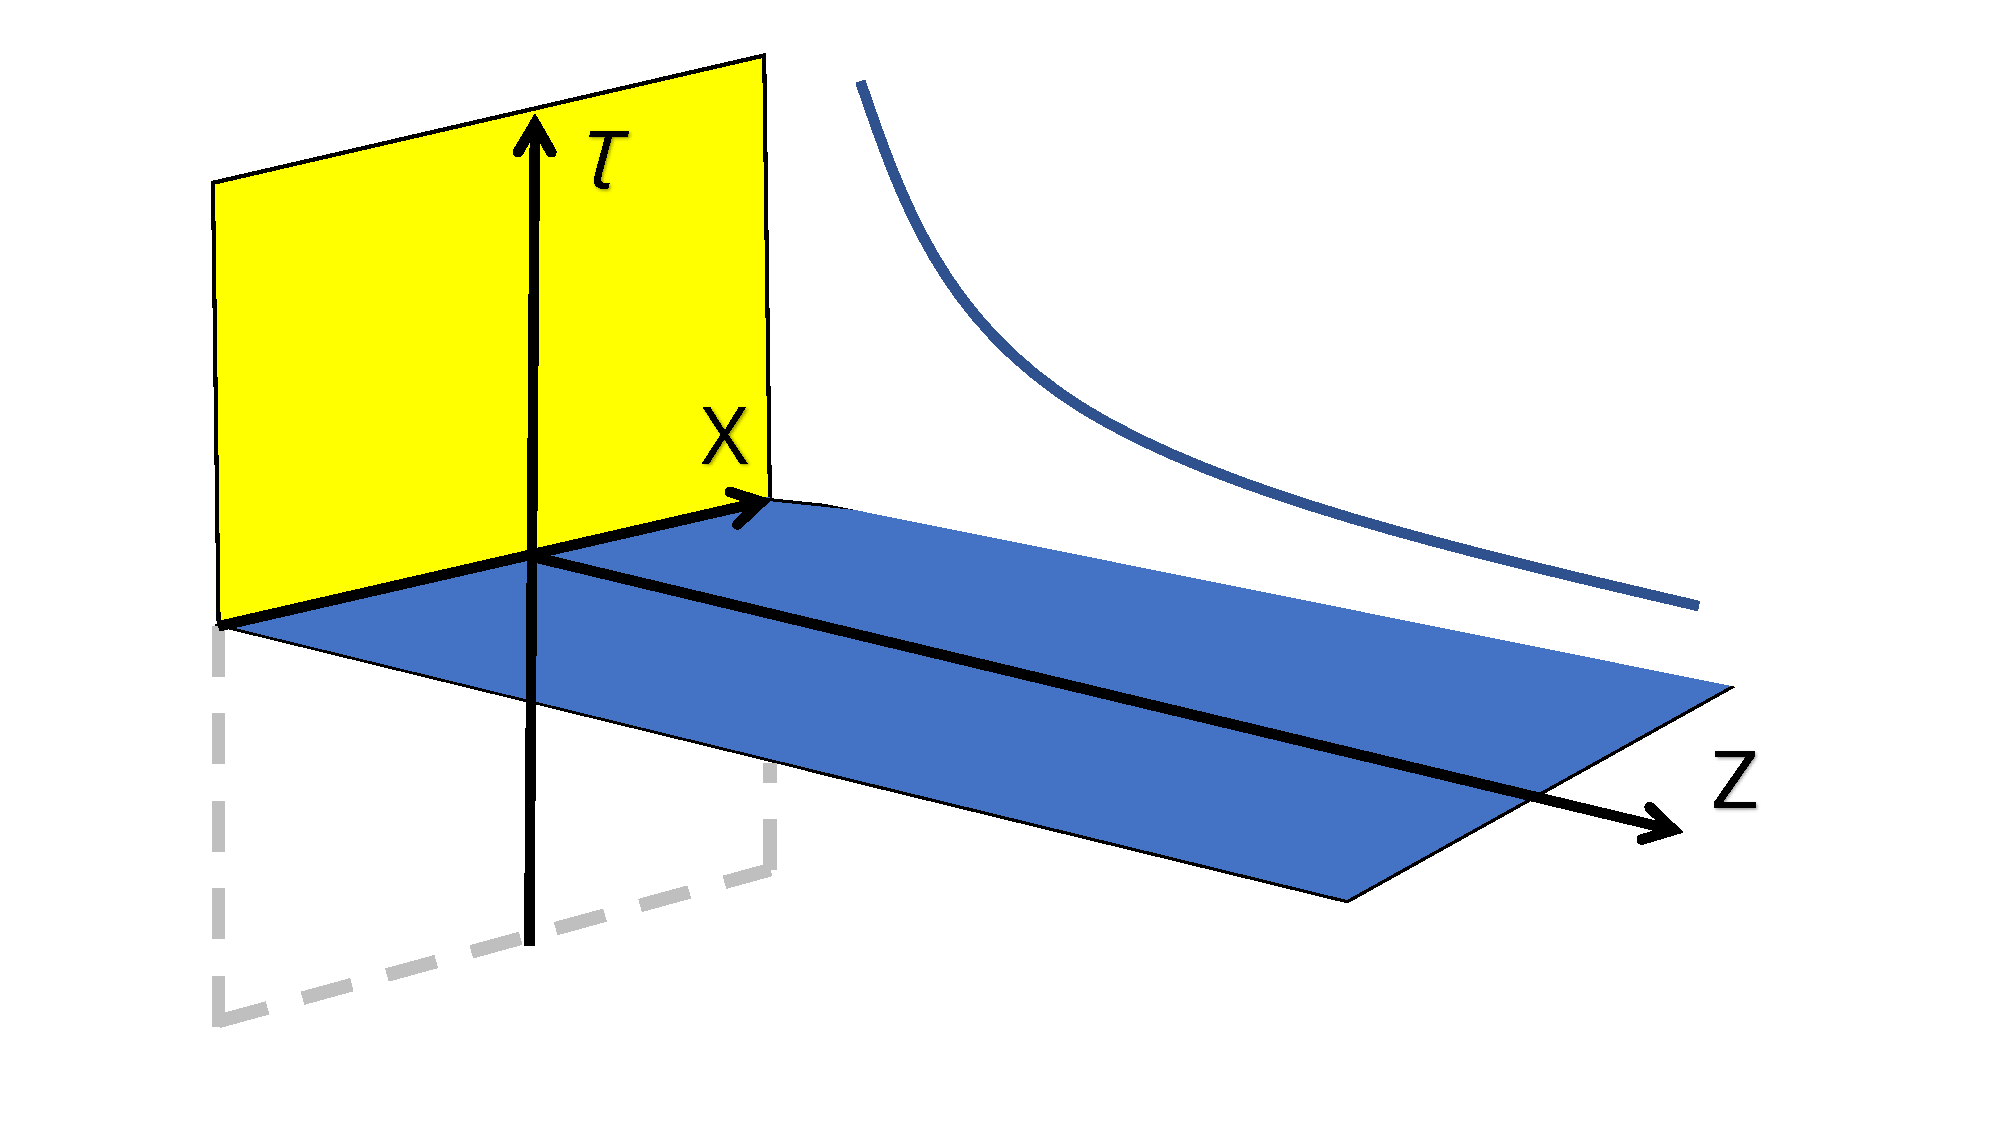
\includegraphics[width=0.7\linewidth]{UHPadsbcft.pdf}
	\label{fig:SQadsbcft}
	\caption{$\zeta$座標に対応する境界付きAdS空間の図。$\IM \zeta=0$面が、AdS/BCFTの処方でNeumann境界条件の課される境界$Q$になる。}
\end{figure}

$c\gg 1$近似を用いると、笠-高柳公式の測地線の候補としては、図(\ref{fig:sqrtsurfacecontraction})のように3つの取り方がある。
\begin{figure}[h]
	\centering
	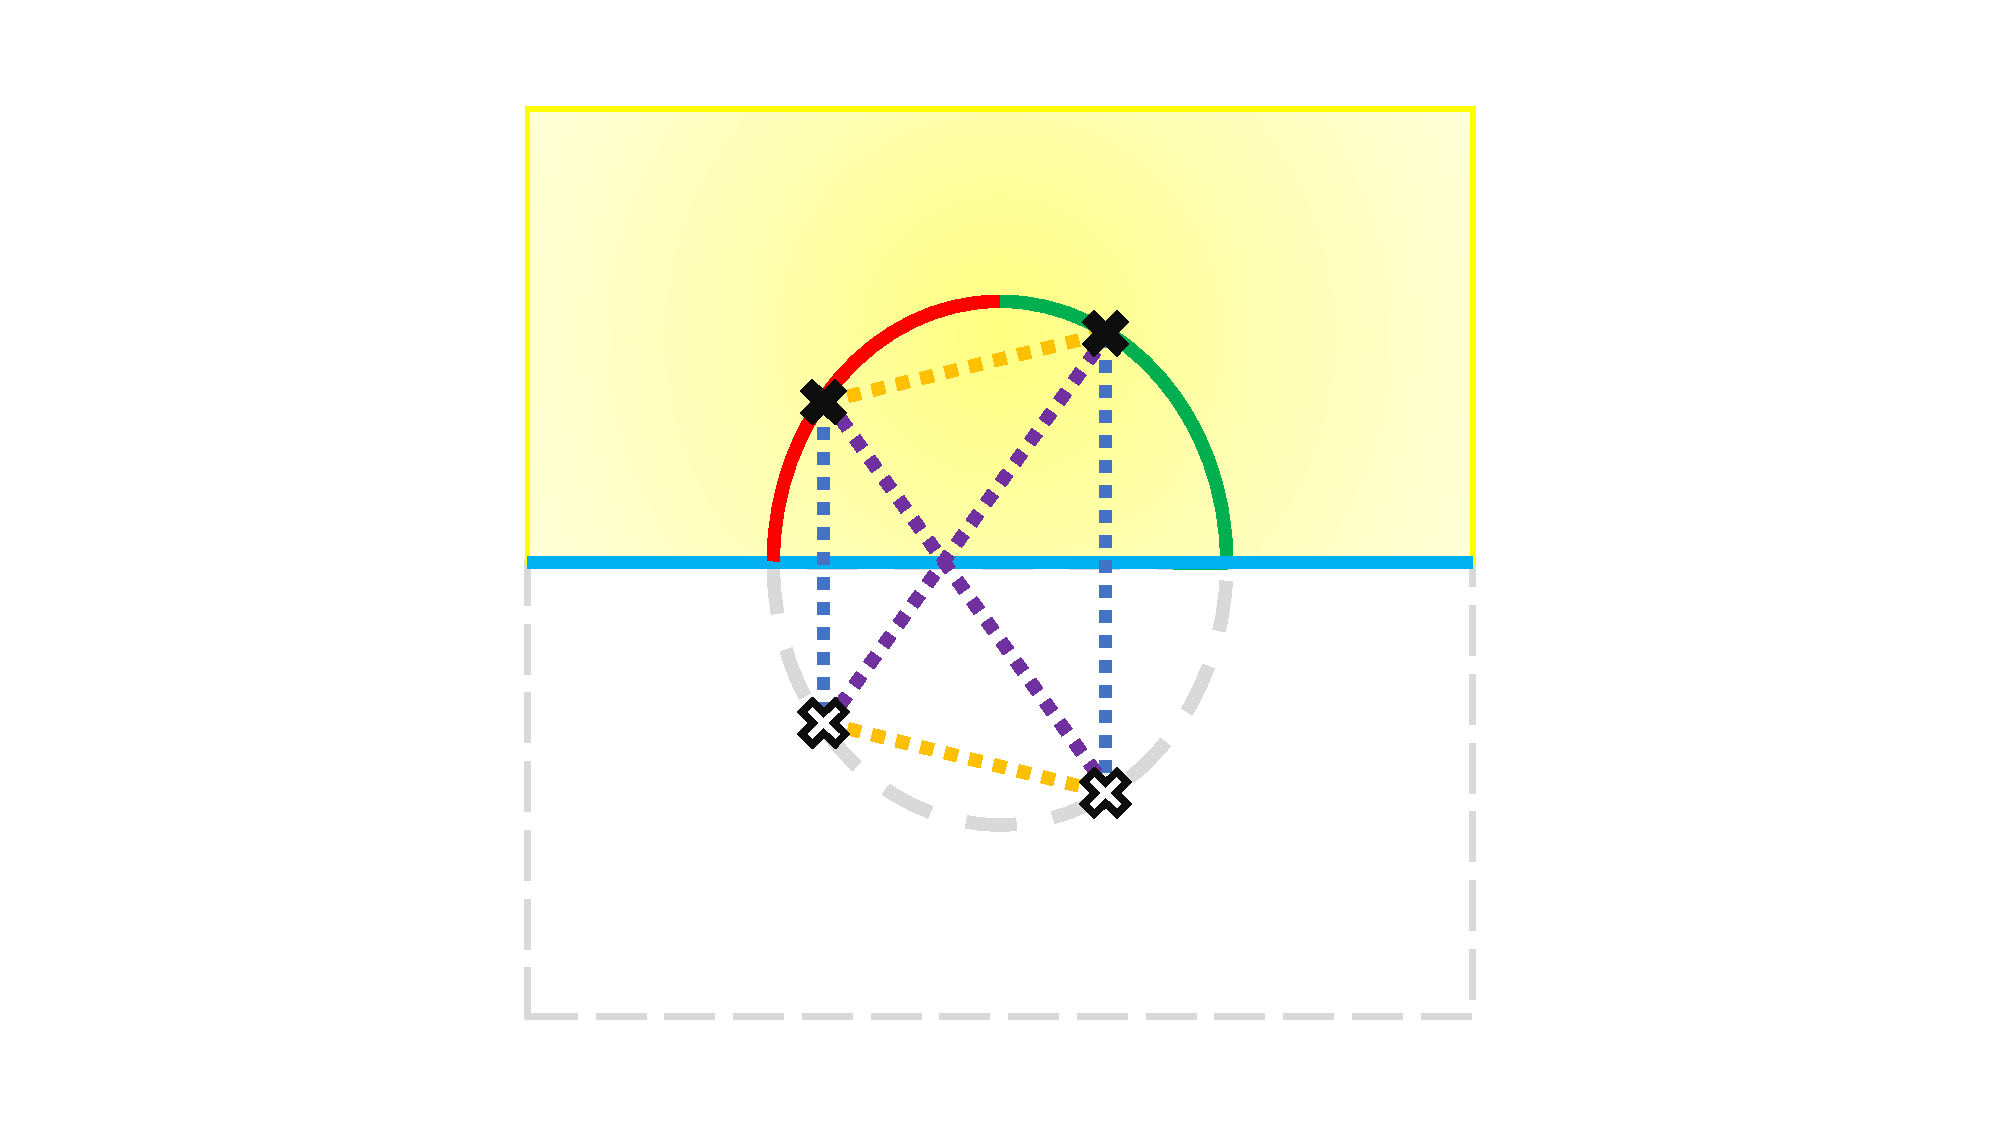
\includegraphics[width=0.7\linewidth]{SQRTsurfacecontraction.pdf}
	\label{fig:sqrtsurfacecontraction}
	\caption{測地線の取り方の図。AdS/BCFTの処方により、AdS空間に対しても``二重化のトリック''の類似を用いることができる。このとき下半平面に鏡像のツイスト演算子があると思って、笠-高柳公式の測地線の長さを計算すればよい。したがって測地線の候補として、オレンジ・紫・青の3つの取り方がある。}
\end{figure}

このときツイスト演算子の4つの挿入点は、必ず半径1の円に内接する四角形を描き、$\zeta_1,\overline{\zeta}_2$と$\zeta_2,\overline{\zeta}_1$を結ぶ測地線が最小となることは無い。したがって、このときも同様に測地線の候補として、$\zeta_1=f(w_1)$と$\zeta_2=f(w_2)$を結ぶ曲線と、$\zeta_1,\zeta_2$がそれぞれの鏡像点$\overline{\zeta}_1,\overline{\zeta}_2$と結ぶ曲線の2種類の取り方があり、それぞれをconnected geodesic, disconnected geodesicと呼ぶことにする。それぞれの測地線に対するエントロピーは
\begin{align}
S^{con}_A&=\frac{c}{6}\log\left(\frac{|f(w_1)-f(w_2)|^2}{\delta_1\delta_2}\right)\\
S^{dis}_A&=\frac{c}{6}\log\left(\frac{4(\IM f(w_1))(\IM f(w_2))}{\delta_1\delta_2}\right)
\end{align}
である。ただし$\delta_i\ (i=1,2)$はPoincare座標での紫外カットオフであり、元の$w$座標に対応する境界付き漸近的AdS空間での紫外カットオフ$\epsilon$との関係は、(\ref{robertsmapz})で$z\sim 0$の極限を考えることで、
\begin{align}
\epsilon |f'(w_i)|=\delta_i\label{cutofftransf}
\end{align}
と関係していることが分かる。

ホログラフィックな共形場理論でのエンタングルメントエントロピーはこれらのうちの小さいほうで求められる。
\begin{align}
S_A(t)=\min \{S^{con}_A(t),S^{dis}_A(t) \}
\end{align}

Dirac場での計算と同様に、$\tau\to it$と解析接続したときの$S^{con}_A(t),S^{dis}_A(t)$の$a\to 0$での近似式を求めると、次のようになる。

\subsub{connected geodesic}
$0<x_1<x_2$のとき
\begin{align}
S_{A}^{con}(t)\sim \frac{c}{6}\log\left\{
\begin{array}{ll}
\bigskip
\dfrac{(x_2-x_1)^2}{\epsilon^2}& (0<t<x_1)\\
\bigskip
\dfrac{2(x_2-x_1)(t-x_1)(x_2-t)}{a\epsilon^2}& (x_1<t<x_2)\\
\bigskip
\dfrac{(x_2-x_1)^2}{\epsilon^2}& (x_2<t)
\end{array}
\right.
\end{align}
$x_1<0<x_2,\ |x_1|<|x_2|$のとき
\begin{align}
S_{A}^{con}(t) \sim \frac{c}{6}\log\left\{
\begin{array}{ll}
\bigskip
\dfrac{(x_2-x_1)^2}{\epsilon^2}& (0<t<-x_1)\\
\bigskip
\dfrac{2(x_2-x_1)(t+x_1)(x_2+t)}{a\epsilon^2}& (-x_1<t<x_2)\\
\bigskip
\dfrac{4(t^2-x_1^2)(t^2-x_2^2)}{a^2\epsilon^2}& (x_2<t)\\
\end{array}
\right.
\end{align}
\subsub{disconnected geodesic}
$|x_1|<|x_2|$のとき
\begin{equation}
S_{A}^{dis} \sim \frac{c}{6}\log\left\{
\begin{array}{ll}
\bigskip
\dfrac{4(x_1^2-t^2)(x_2^2-t^2)}{a^2\epsilon^2}& (0<t<|x_1|)\\
\bigskip
\dfrac{4|x_1|(x_2^2-t^2)}{a\epsilon^2}& (|x_1|<t<|x_2|) \\
\bigskip
\dfrac{4|x_1||x_2|}{\epsilon^2}& (|x_2|<t)
\end{array}
\right.
\end{equation}

したがって$t\to\infty$での$S_A$は
\begin{align}
S_A(t\to\infty)\sim \left\{ \begin{array}{ll}
\bigskip
\min\left\{ \dfrac{c}{3}\log\dfrac{|x_2-x_1|}{\epsilon},\  \dfrac{c}{6}\log\dfrac{4|x_1||x_2|}{\epsilon^2} \right\} & (x_1x_2>0) \\
\bigskip
\dfrac{c}{6}\log\dfrac{4|x_1||x_2|}{\epsilon^2} & (x_1x_2<0) 
\end{array}\right.
\end{align}
となる。

\subsub{数値計算}
上の計算を数値計算したものがグラフ\ref{fig:sh005}である。$a=0.05$で$S_A(t)$と真空のEE$S_\text{vac}=(c/3)\log(L/\epsilon)$の差を計算しており、左図は部分系$[50,150]$,右図は$[-20,50]$にとった場合である。青線がconnected geodesicに対応するグラフで、赤線がdisconnecetd geodesicに対応するグラフであり、$S_A(t)$は2つの最小値である。
\begin{figure}[h]
	\centering
	\begin{tabular}{c}
		\begin{minipage}{0.50\hsize}
			\centering
			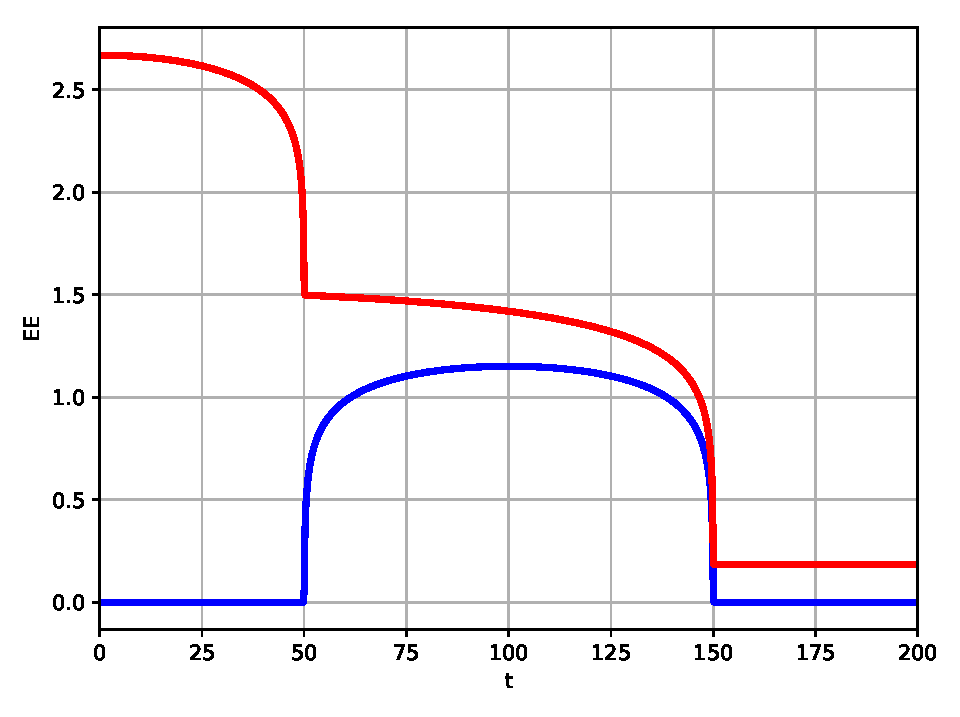
\includegraphics[width=\linewidth]{sh005_50_150.pdf}
		\end{minipage}
		\begin{minipage}{0.50\hsize}
			\centering
			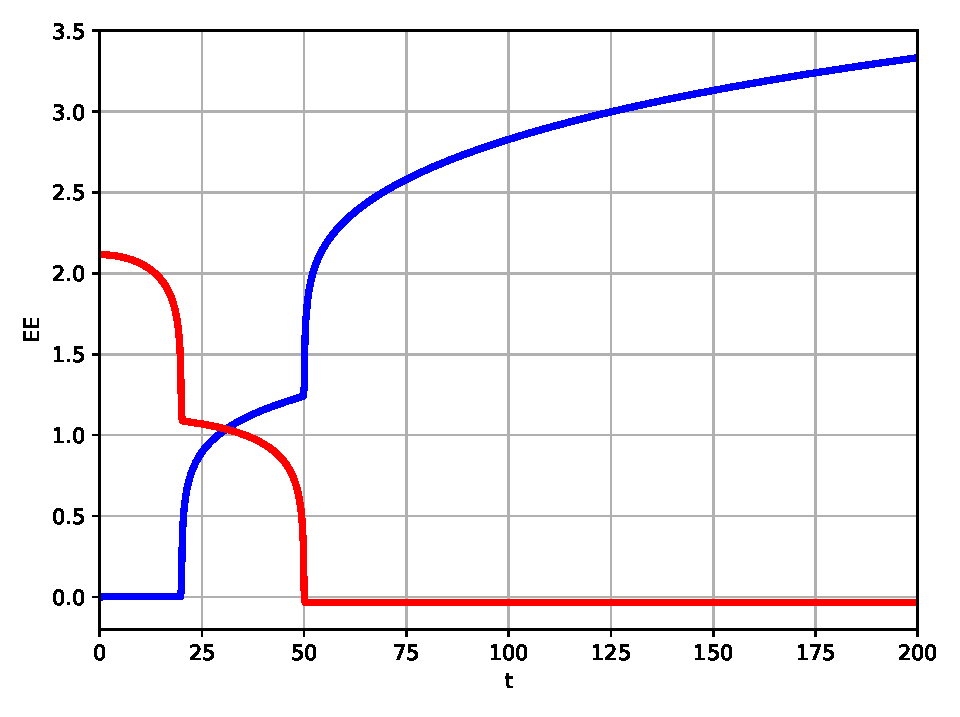
\includegraphics[width=\linewidth]{sh005_20_50.pdf}
		\end{minipage}
	\end{tabular}
	\caption{重力双対を持つ共形場理論の真空を分離クエンチしたときのEEのグラフ。横軸は時間$t$で、縦軸は真空の寄与を引いたEE $S_A(t)-S_\text{vac}$をプロットしている。青線がconnected geodesicに対応するグラフで、赤線がdisconnecetd geodesicに対応するグラフである。}
	\label{fig:sh005}
\end{figure}
この結果も準粒子描像に当てはまっている。

\subsection{AdS側での解釈}
ホログラフィックな共形場理論でのエンタングルメントエントロピー$S_A$をAdS空間の測地線の長さとして求めたが、ここでは$S_A$の振る舞いをAdS側の言葉で解釈してみる。

AdS/BCFTの処方により、上半平面$\zeta$の双対となるAdS時空をPoincare座標
\begin{align}
ds^2 = R_A^2 \frac{d\eta^2+d\zeta d\overline{\zeta}}{\eta^2},\ \IM \zeta>0
\end{align}
にとる。このとき(\ref{robertsmap1})(\ref{robertsmap2})(\ref{robertsmapz})の変換をすると、$w=x+i\tau$座標のホログラフィック共形場理論に対応する境界付きAdS空間の計量は、Feffermann-Graham計量の形で与えられ、
\begin{align}
ds^2&=R_A^2 \left( \frac{dz^2}{z^2}+L(w)dw^2+\overline{L}(\overline{w})d\overline{w}^2+\left( \frac{1}{z^2}+ z^2L(w)\overline{L}(\overline{w})\right)dwd\overline{w}  \right)\\
L(w)&=\frac{3(f'')^2-2f'f'''}{4f'^2}=\frac{3a^2}{4(w^2+a^2)^2}
\end{align}
である。

また、$(\zeta,\overline{\zeta},\eta)$と$(w,\overline{w},z)$は
\begin{align}
\zeta&=i\sqrt{\frac{w+ia}{w-ia}}\left( 1-ia\frac{2z^2(\overline{w}-ia)}{4|w^2+a^2|^2+z^2|2w+ia|^2} \right)\\
\eta&=a\frac{4z|w+ia|^{3/2}|w-ia|^{1/2}}{4|w^2+a^2|^2+z^2|2w+ia|^2}
\end{align}
で関係しており、上半分のPoincare座標では$\IM \zeta=0$にあったboundary surfaceは、この変換によって$Q=\{(x,\tau,z)\mid x=0, \tau\in [-a,a], z>0 \}$面に移ることが分かる。

このとき、計量$ds^2$の体積要素は
\begin{align}
\sqrt{\det(ds^2)}=\frac{R_A}{z^3}\sqrt{ (z^4L^2-1)(z^4\overline{L}^2-1)+z^4(L-\overline{L})^2}
\end{align}
である。

「$x\sim a$かつ$\tau=0$」あるいは「$x=0$かつ$\tau\sim a$」では$L\sim \frac{3}{16 a^2}$となるから、
\begin{align}
\sqrt{\det(ds^2)}\sim \frac{R_A}{z^3}\left|1-\left(\frac{\sqrt{3}z}{4a}\right)^4\right|
\end{align}
である。Poincare座標の体積要素は$R_A/z^3$であるから、虚時間のセットアップにおいて計量は「$x\sim a$かつ$\tau=0$」あるいは「$x=0$かつ$\tau\sim a$」で大きく曲がっていることが分かる。つまり$ds^2$はその境界$Q$付近で大きく曲がっており、境界$Q$はAdS$_3$時空のPoincare座標に存在する``非常に重い物体''として解釈できる。

したがって、Lorentz時間のセットアップを考えた時には、HRT公式から測地線は計量の$\det$の大きくなる境界近くに張り付くようになり、下図のようになる。
\begin{figure}[H]
	\centering
	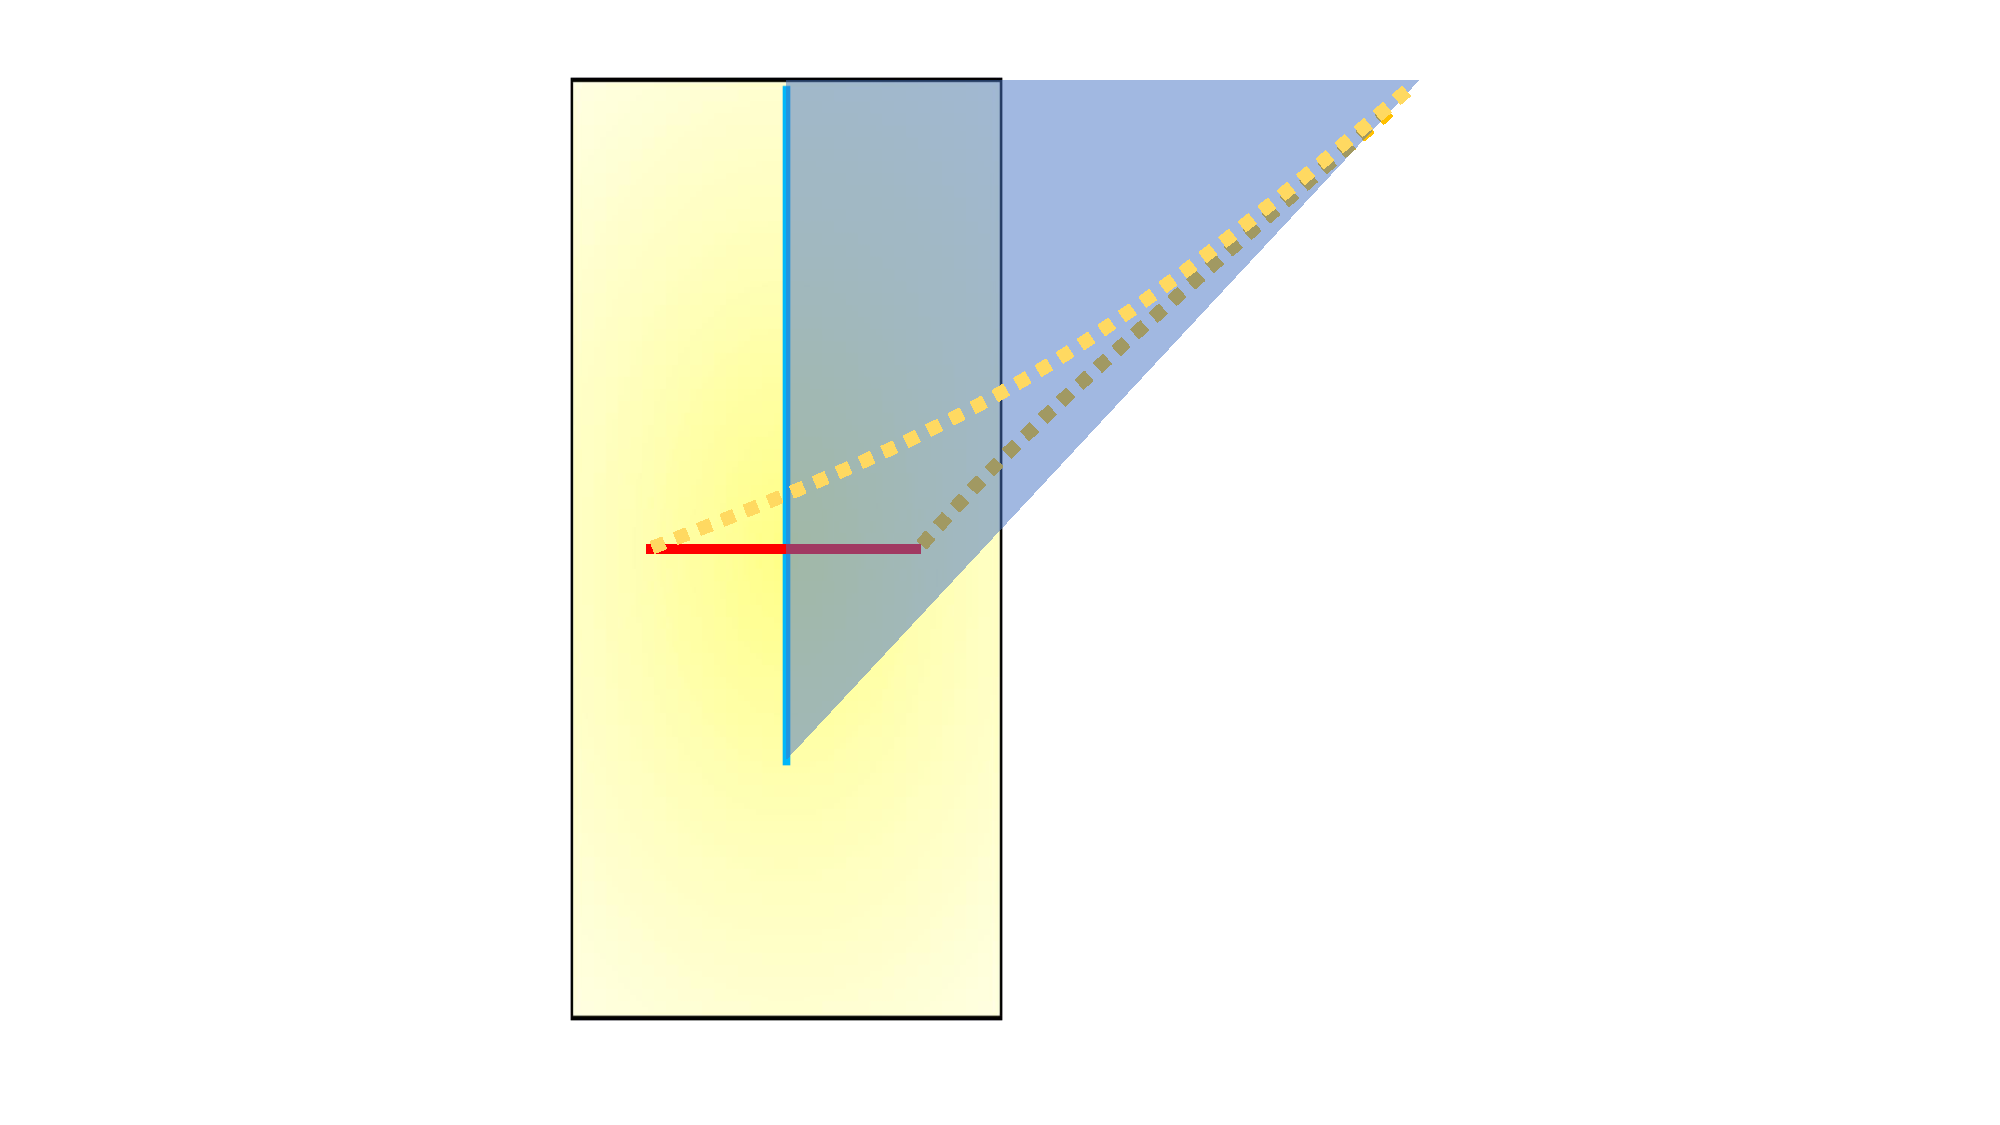
\includegraphics[width=0.7\linewidth]{SQgeod.pdf}
\end{figure}

したがって境界をまたぐ部分系で$t\to \infty$でconnected geodesicの長さが$\log$発散したのはこの境界によって障害が生まれたためであると考えられる。
